\documentclass{article}
\usepackage[utf8]{inputenc}
\usepackage{amssymb}
\usepackage{graphicx}
\usepackage{geometry}
 \geometry{
 a4paper,
 total={170mm,257mm},
 left=20mm,
 top=20mm,
 }
\usepackage[colorlinks=true,linkcolor=blue]{hyperref}%
\title{Gradient Descent Very Brief Review}
\author{Tomer Bar-Natan \\205679863 \and Gilad Deutch \\311151138 \and Nadav Magar \\ 318635646}
\date{March 14, 2023}

\begin{document}
\maketitle

\begin{abstract}
	Gradient descent is an iterative optimization algorithm for finding the local minimum of a function.
	It and its variants are with no doubt the most common optimization algorithms which are used in
	ML.
\end{abstract}

\section{Introduction}
Optimization refers to the task of minimizing/maximizing
an objective function $f(x)$ parameterized
by $x$. In machine/deep learning terminology, it's the task of minimizing the cost/loss function
$\mathcal{L}(\theta)$ parameterized by the model's parameters $\theta \in \mathbb{R}^{d}$.
This objective function might be represented in
many ways - it could be a simple linear function such that $\theta$ is just one matrix, as well as a 175B
parameters transformer architecture, such that $\theta$ is a collection of large number of matrices and bias
terms. Optimization algorithms (in the case of minimization) have one of the following goals:

\begin{itemize}
	\item Find the global minimum of the objective function. This is feasible if the objective function is
	      convex, i.e. any local minimum is a global minimum.
	\item Find the lowest possible value of the objective function within its neighborhood. That's usually the
	      case if the objective function is not convex as the case in most deep learning problems.

\end{itemize}

\section{Algorithm}
Let's denote our objective function by $\mathcal{L}$ (it is often referred to it as the loss function), and let's say
it is parameterized with some parameters which we will denote with $\theta$.
Additionally, let's denote an
additional hyperparameter the algorithm uses, called the \emph{learining rate},
with $\eta$.  The Vanilla Gradient
Descent Algorithm suggests following these following steps:

\begin{enumerate}
\item Start by Randomly initialize values for $\theta_{0}$
	\item Update $\theta$ values: $\theta_{t+1}=\theta_{t}-\eta\nabla L(\theta)$
	\item Repeat until the slope is approximately flat. Namely,
	      $\frac{\partial\mathcal{L}(\theta)}{\partial\theta}\approx 0$
\end{enumerate}

\subsection{Learning Rate}
How big the steps gradient descent takes into the direction of the local minimum are determined by the
learning rate, which figures out how fast or slow we will move towards the optimal weights. To illustrate
the effects of a wrong/right choice of the learning rate, Figure \ref{fig:lr} is attached.

\begin{figure}[h!]
	\centering
	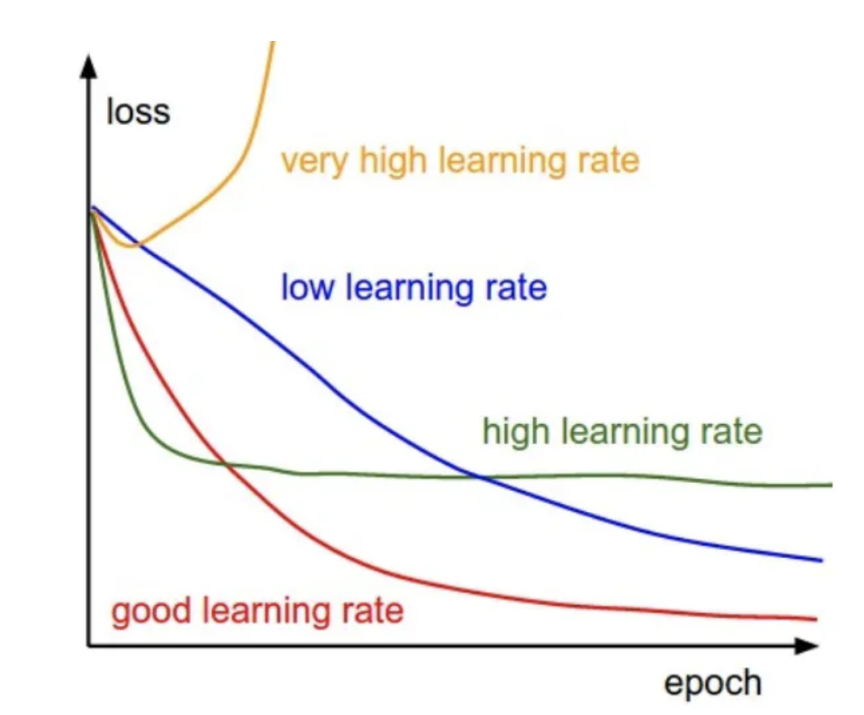
\includegraphics[scale=0.75]{figure.png}
	\caption{Effects of using too large/small learning rate while applying the GD algorithm}
	\label{fig:lr}
\end{figure}

\end{document}